\documentclass[11pt]{article}
\usepackage{graphicx}
\usepackage{float}

\begin{document}
\title{Lesson 21: Boundary Value Problems}
\author{Colt Bradley}
\date{}
\maketitle

\section{Part 1}

In this first part, we use the relaxation equation defined in the instructions, repeating it until a certain error threshold is allowed between subsequent sweeps. The error threshold is noted in each graph, and in the comment below each graph the number of sweeps it too to meet that threshold is noted. 

Though there is a significant step difference in the last three graphs, they look fairly similar. We need to judge the trade off between having a more exact result and the time it takes to compute that result. If we only need the graph, then perhaps graph (c) would be enough. 

\begin{figure}[H]
\centering
\begin{tabular}{cc}
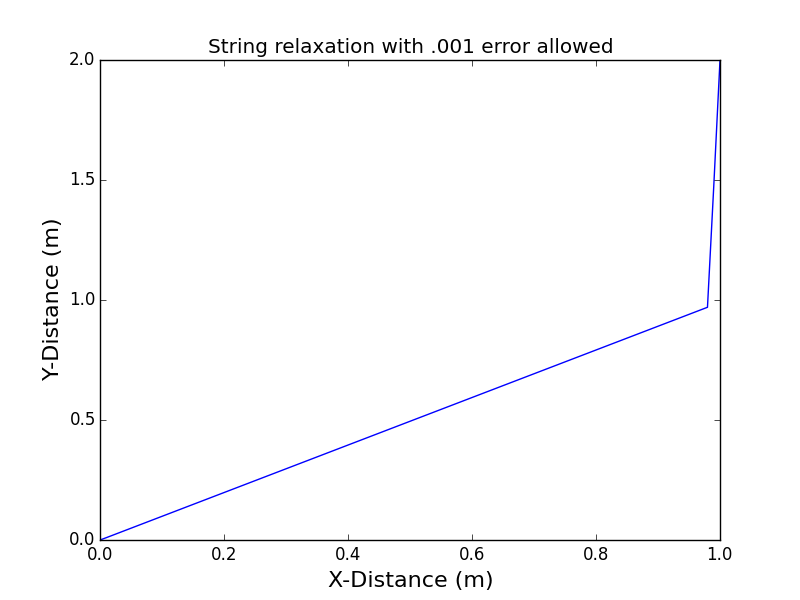
\includegraphics[scale=.3]{1_relaxation(001).png} & 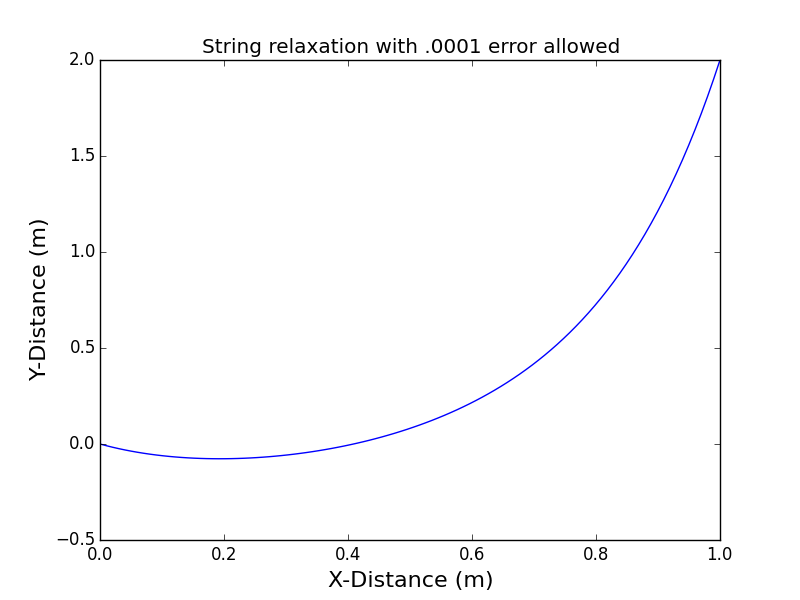
\includegraphics[scale=.3]{1_relaxation(0001).png} \\
(a) After 1 sweep & (b) After 1781 sweeps \\[6pt]


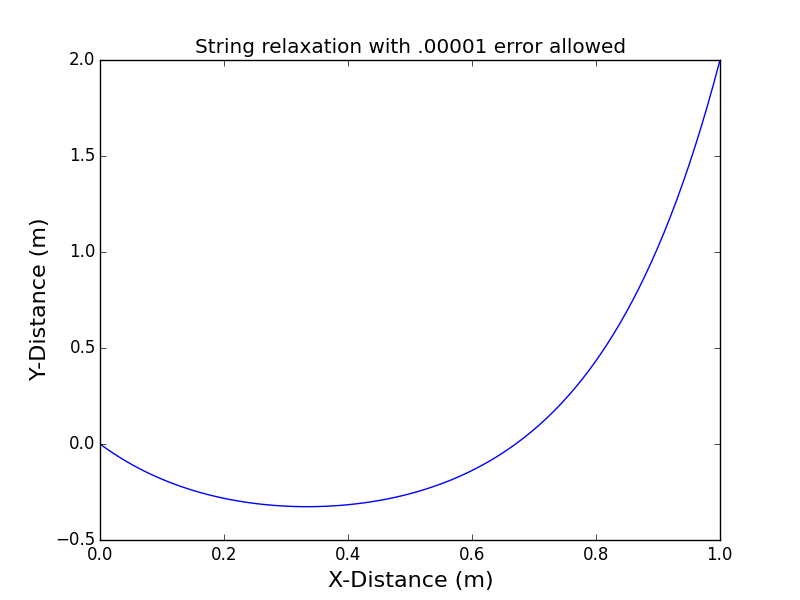
\includegraphics[scale=.3]{1_relaxation(00001).png} & 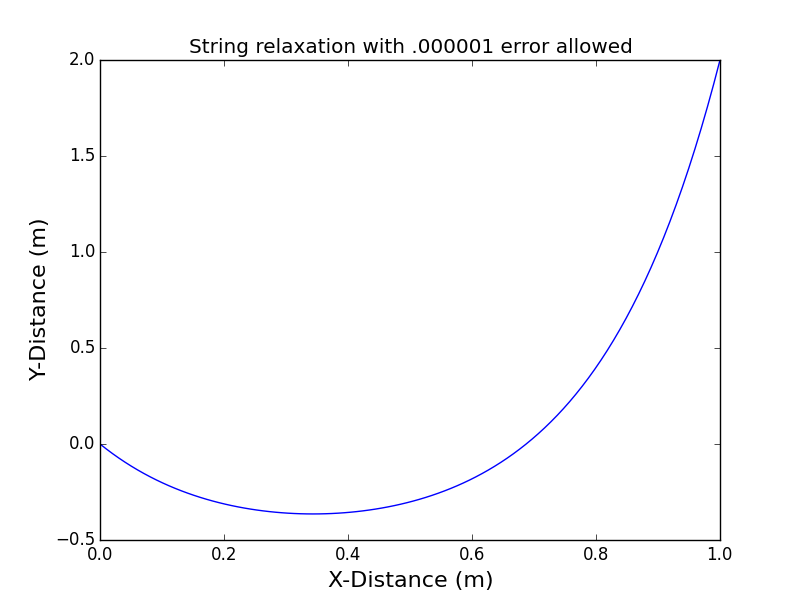
\includegraphics[scale=.3]{1_relaxation(000001).png}\\
(c) After 8709 sweeps & (d) After 16861 sweeps \\[6pt]

\multicolumn{2}{c}{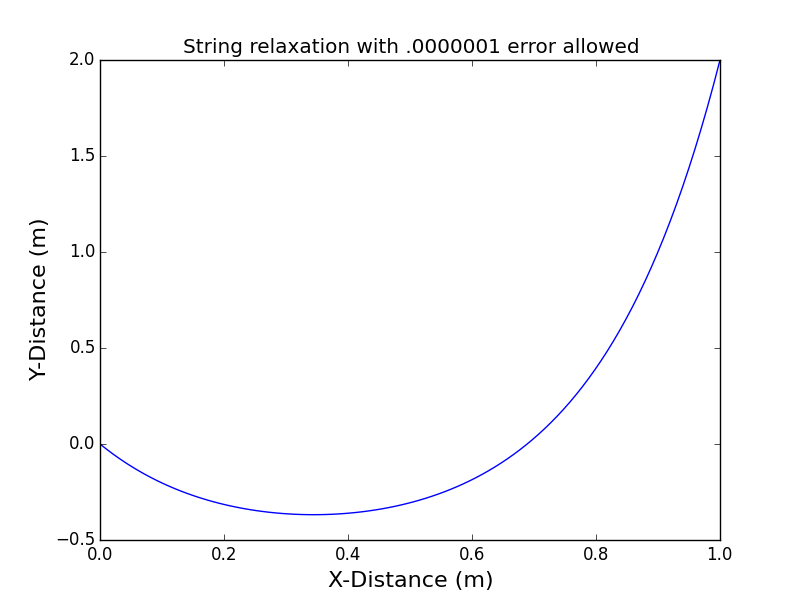
\includegraphics[scale=.3]{1_relaxation(0000001).png}}\\
\multicolumn{2}{c}{(e) After 25139 sweeps} \\[6pt]
\end{tabular}
\caption{Various plots for $\cos (6\pi t) e^{-t^2} $}
\end{figure}

\section{Part 2}

\section{Part 3}

\section{Code}
\subsection{Part 1 Code}
\begin{verbatim}
#Colt Bradley
#4.18.16
#Lesson 21: Boundry Value Problems

###############################################################################
#Import Modules and define functions
###############################################################################
import numpy as np
import pylab as py

###############################################################################
#Part 1
###############################################################################

#define values
k=5.
x_0=0.
x_f=1.
y_0=0.
y_f=2.
N=100.
change = 10.
ch=[]
steps=0
h = (x_f-x_0)/N
X=np.linspace(0,1,100)
Y=np.zeros(N)
Y[0]=y_0
Y[-1]=y_f
for i in range(len(Y+1))[1:-1]:
    Y[i]=Y[i-1]+h
ch.append(Y[50])

while change>.0000001:    
    Y[1:-1] = .5*(Y[:-2]+Y[2:])-(k*h**2)/2.*np.sqrt(1+((Y[:-2]-Y[2:])**2)/(2*h)**2)
    ch.append(Y[50])
    change = abs(ch[-1]-ch[-2])
    steps= steps+1

print steps

py.close()
py.plot(X,Y,"b")
py.title("String relaxation with .0000001 error allowed")
py.xlabel("X-Distance (m)",fontsize = 16)
py.ylabel("Y-Distance (m)",fontsize = 16)
py.savefig("1_relaxation(.0000001).png")
py.show()
\end{verbatim}
\subsection{Part 2 Code}

\subsection{Part 3 Code}


\end{document}